\chapter{Plant functional types mapping}
We proposed a combined machine learning approach with a deep convolutional neural network (CNN) to monitor forest utilization toward Sustainable Development Goals (SDGs) for data-scarce regions. First, we employed the Random Forest (RF) classifier using Google Earth Engine (GEE) for forest mapping. Then, we designed a deep CNN architecture that works for tree species/age mapping from coarse and polygonal ground-truth data. The proposed network has U-shape and comprises 3D Atrous Convolutions. The model was optimized by a weighted cross-entropy loss function. We trained the model with times-series Sentinel 1, 2, and Digital Elevation Model (DEM) data with sparse annotations. Our proposed models achieved 94.5\% overall accuracy (OA) for forest mapping, 77.80\% (OA) for tree species, and 81.74\% (OA) for tree age classification, respectively in Ena city, Japan. The outcome of our study indicates the potential of remote sensing and machine learning in monitoring forest development, conservation, and utilization toward SDGs from coarse ground-truth data. Our source code for the implementation is available at: \url{https://github.com/anhp95/forest_attr_segment}
\renewcommand{\headrulewidth}{0pt}
\lhead[\thepage]{\leftmark}
\rhead[\leftmark]{\thepage}
\cfoot[]{}

\section{Introduction}
Forest plays an important role in achieving SDG15 and mitigating the climate change at the global level. With the help of remote sensing and state-of-the-art machine learning algorithms, mapping the forest area with tree species/age could contribute to monitoring the forest-related SDG issues such as SDG indicators 15.1.1, 15.2.1, 15.4.2. \par
Forest mapping is a well-known task in land-cover/ land-use classification problems. However, tree species/age map is obtained at the cost of much higher complexity. In the previous studies in tree species/age classification, either high-resolution input \citep{schiefer2020mapping,la2021multi} or ground-truth data (point-level) is commonly used. These materials are considered to be expensive, time-consuming to collect, and rarely available in specific regions (e.g., developing regions). Therefore, in this chapter, we present a methodology to help monitor forest areas, tree species/age from coarse annotations and free remote sensing data. Firstly, we classify forest area using RF classifier. Subsequently, we designed a deep CNN architecture for tree species/age segmentation. We demonstrated that our proposed approach is considered to be useful for data-scarce regions. \par
The paper outline is described as follows. Section \ref{chap5_data} presents the study area and data used in the paper. Section \ref{chap5_method} provides the overall methodology and the experimental results in the study area are introduced in Section \ref{chap5_result}. Finally, the conclusion of the paper and the future works is remarked in Section \ref{chap5_conclusion}. \par

\section{Data} \label{chap5_data}
\subsection{Study area}
The study area is Ena city, located in the southeastern part of Gifu prefecture, middle of Japan. The total area of Ena city is approximately 504 km2 with an elevation of 282 meters. The annual temperature of the city ranges from 2 °C to around 26.4 °C. According to the statistics of the local government, 60\% of the forest in Ena is artificial forest which is dominated by Chamaecyparis obtusa. Here, the forest plays a vital role in timber production, water-related disaster prevention and CO2 sequestration. \par

\begin{figure}[p]
    \centering
    \begin{subfigure}{\textwidth}
        \centering
        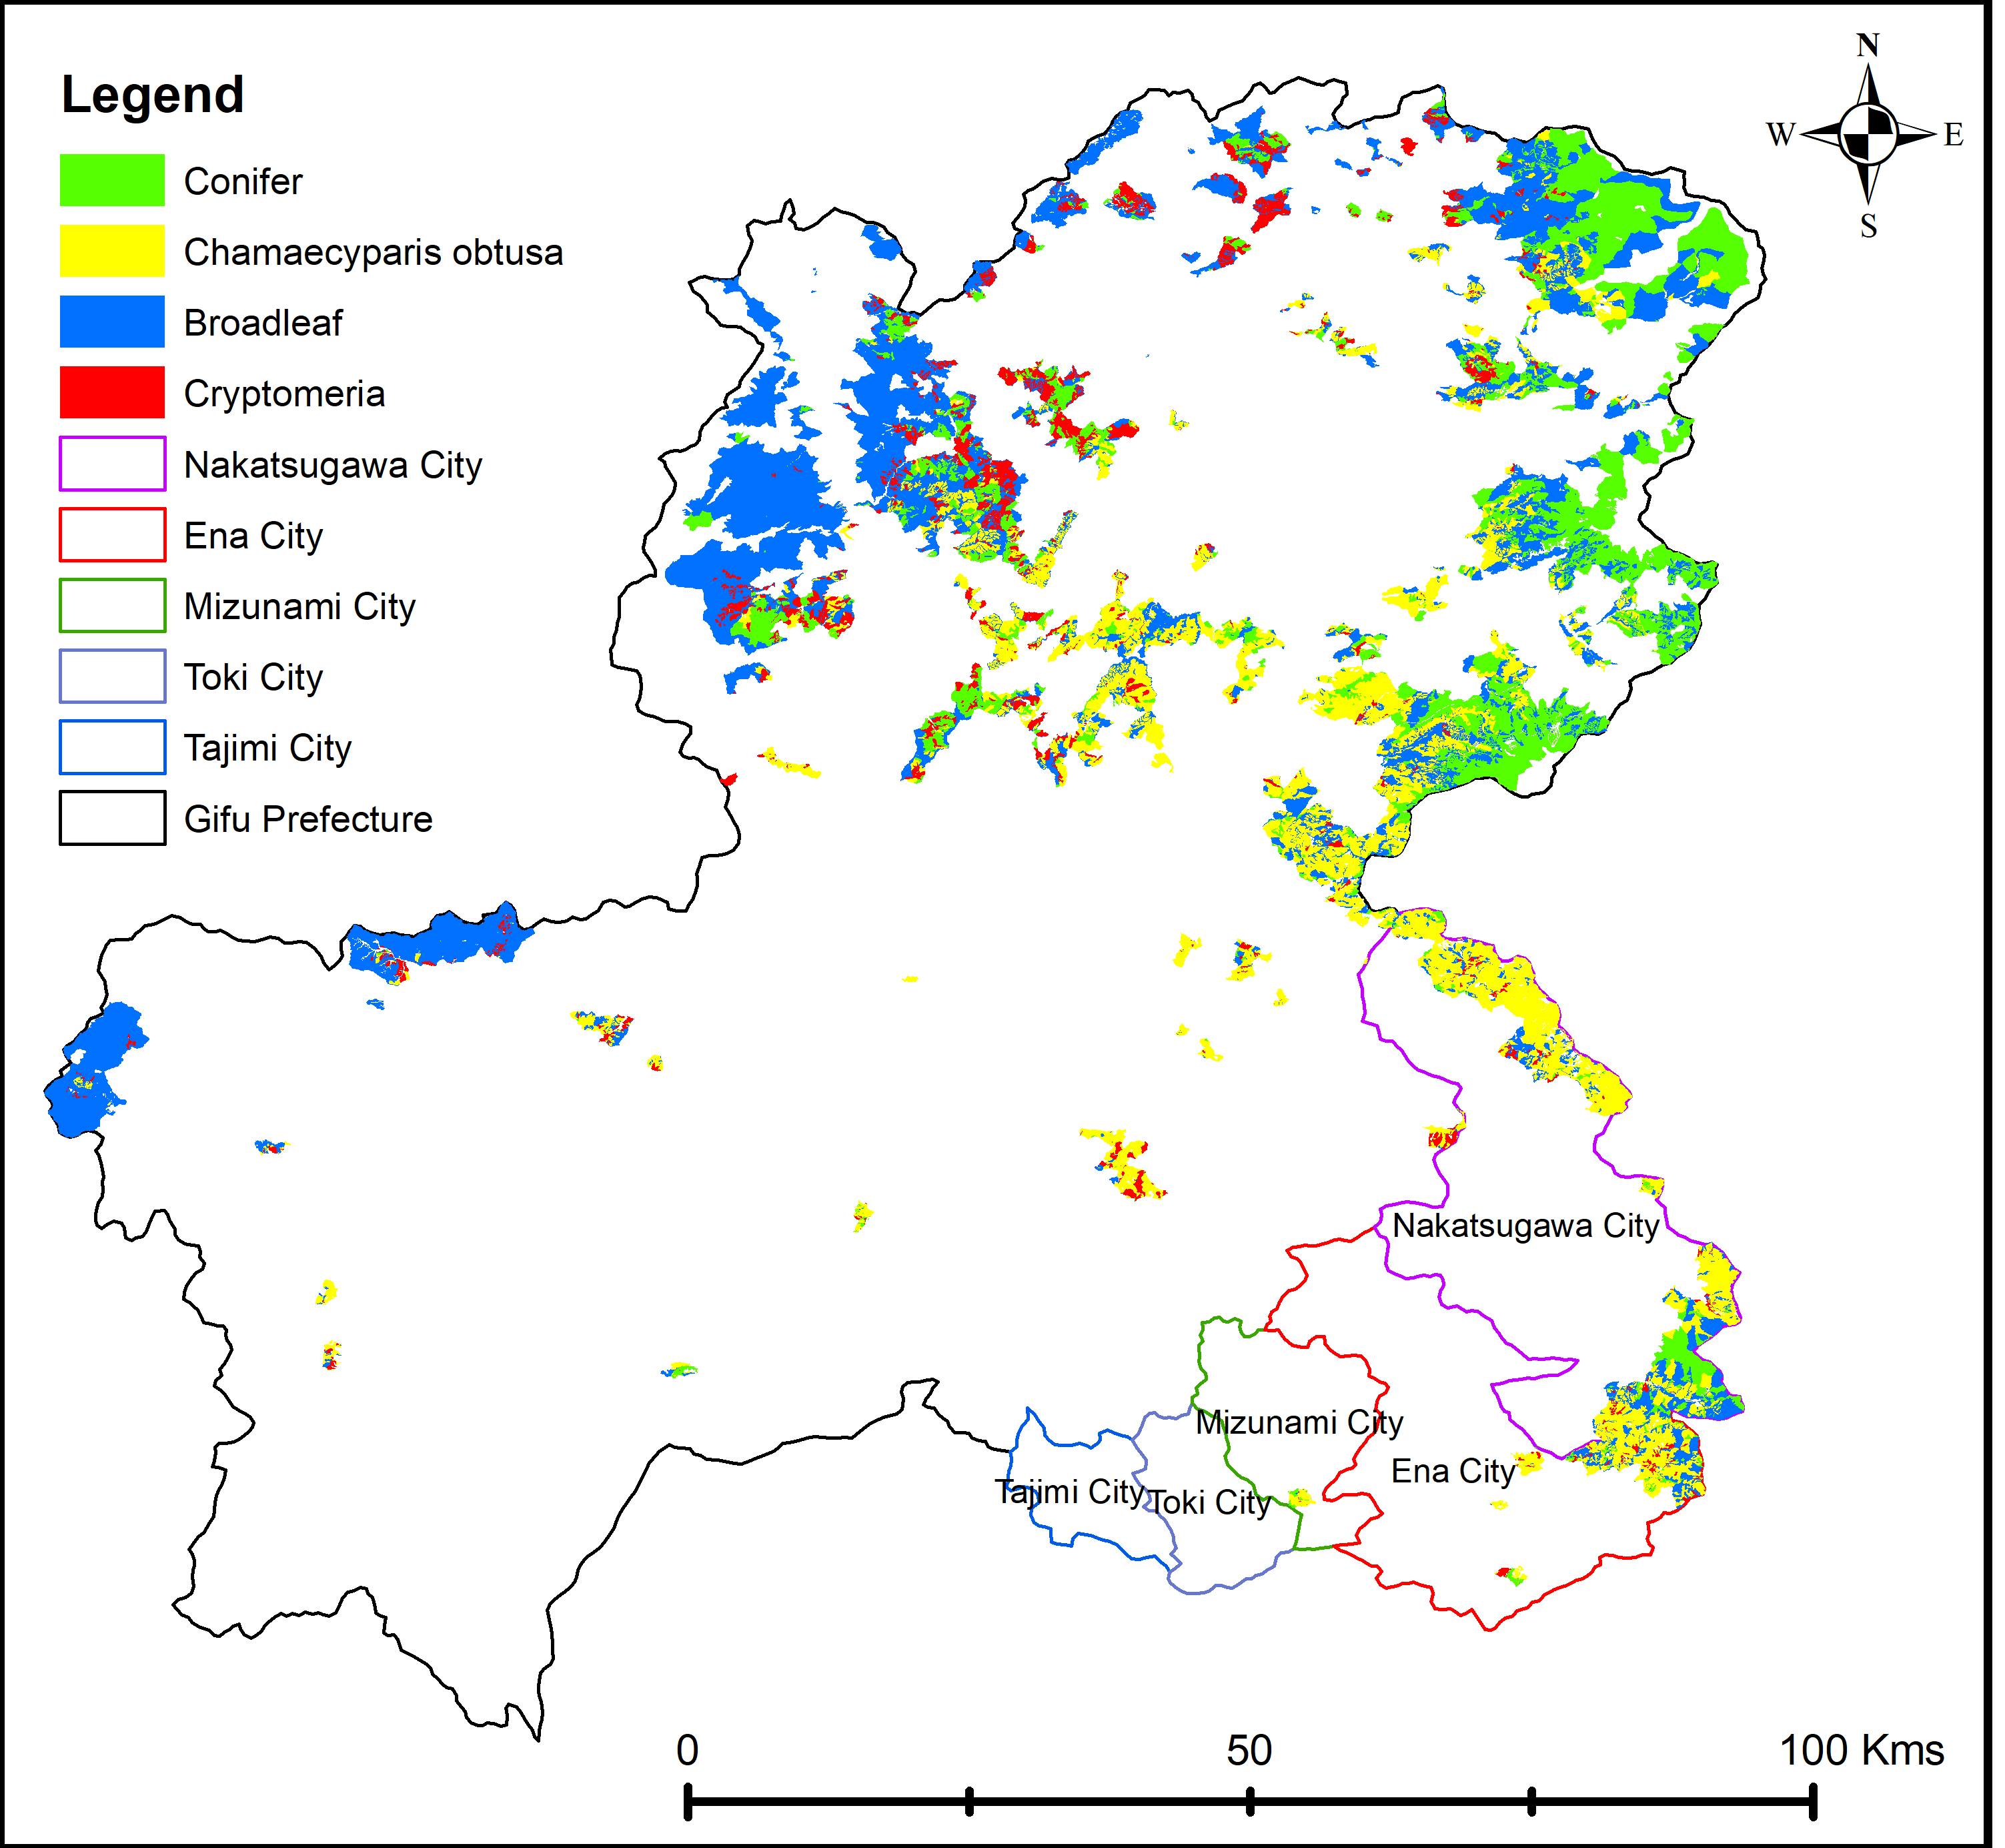
\includegraphics[width=\textwidth]{figs/chap5/studyarea.png}
        \caption{Annotations of national forest in Gifu prefecture (black boundary)}
        \label{fig:chap5_studyarea}
    \end{subfigure}

    \begin{subfigure}{.5\textwidth}
      \centering
      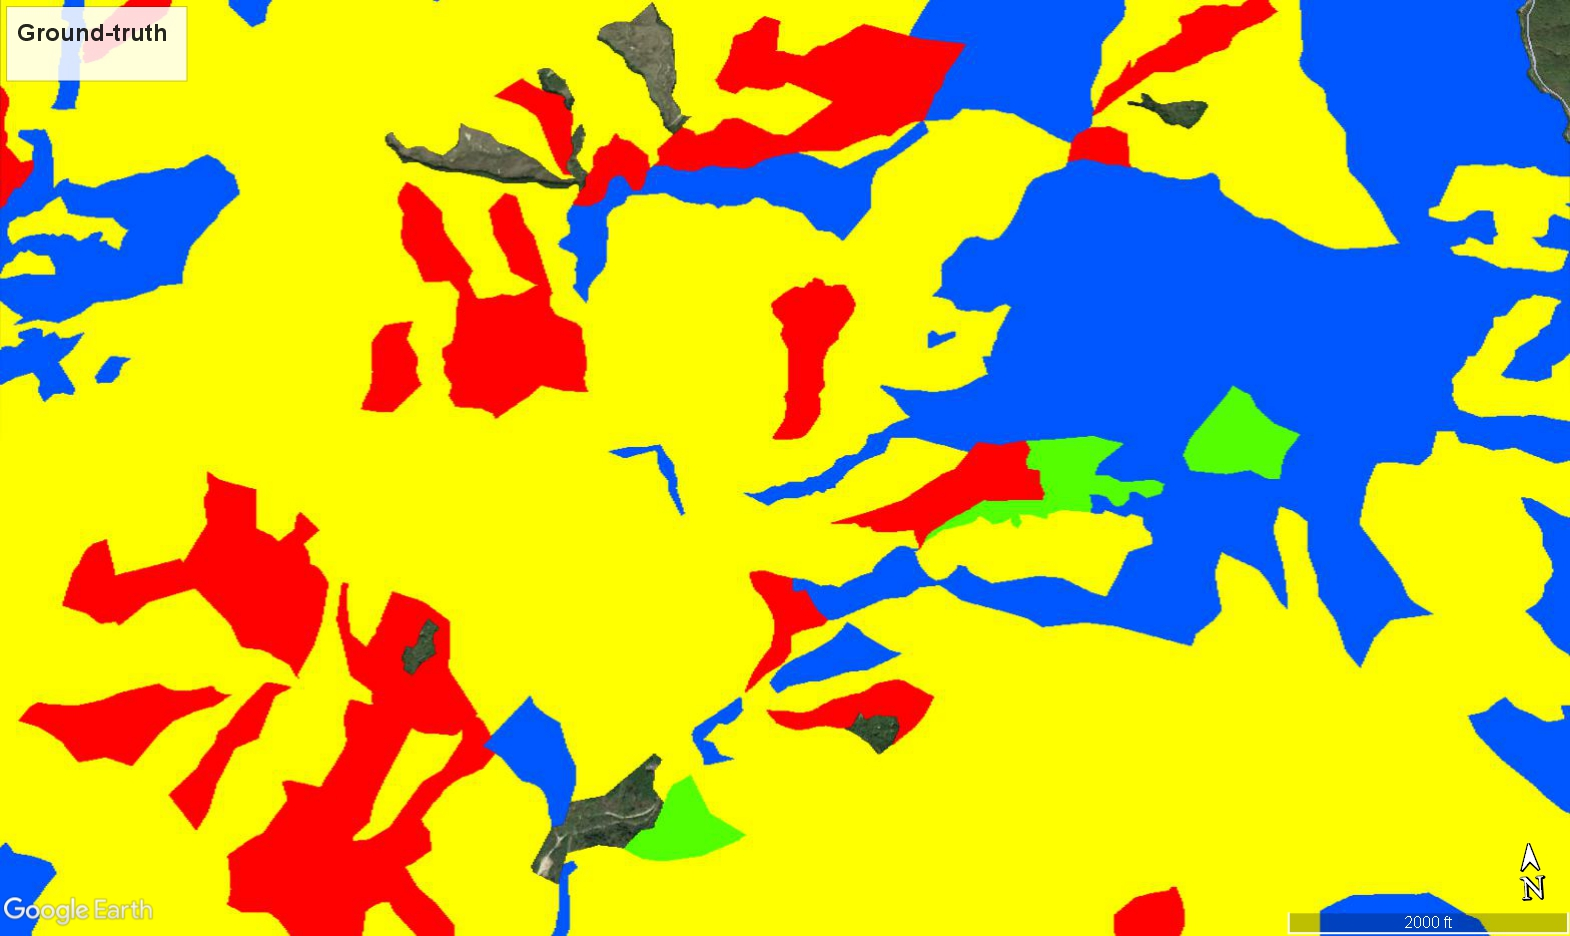
\includegraphics[width=\textwidth]{figs/chap5/gt-ge.jpg}
      \caption{Example of annotated area}
      \label{fig:chap5_gtge}
    \end{subfigure}%
    \begin{subfigure}{.5\textwidth}
      \centering
      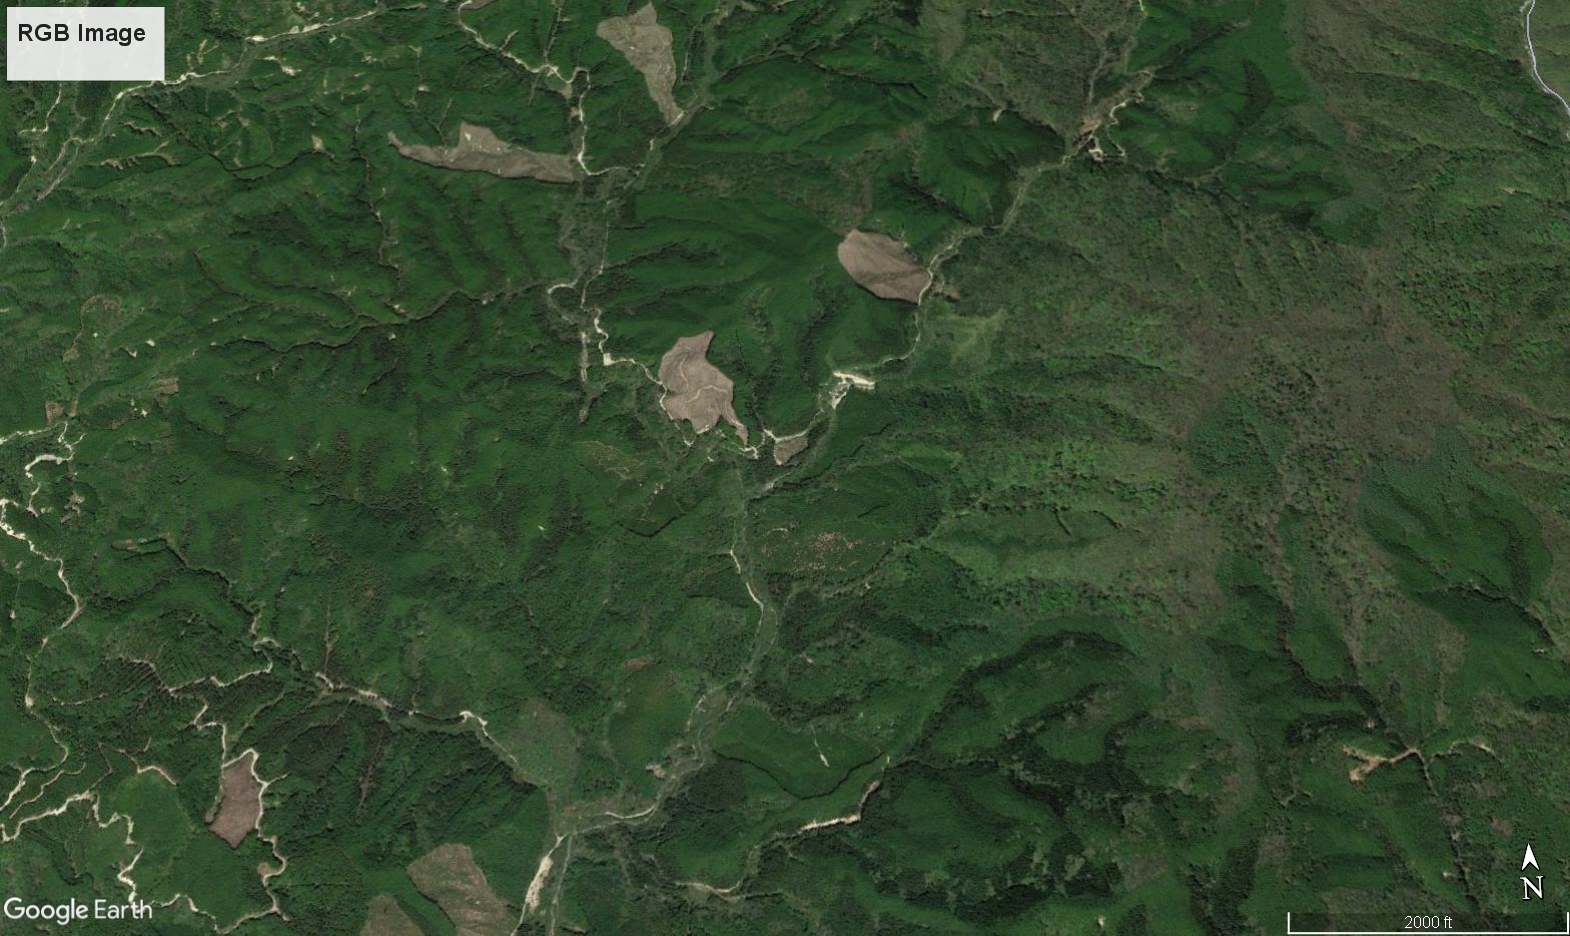
\includegraphics[width=\textwidth]{figs/chap5/gt-rgb.jpg}
      \caption{The corresponding RGB image}
      \label{fig:chap5_gtrgb}
    \end{subfigure}
    \caption[Study area and annotated data]{(a) The designated study area outlined in red is Ena city, (b) demonstrates coarse annotations as an illustrative example, and (c) showcases the corresponding RGB image sourced from Google Earth.}
    \label{fig:chap5_studyarea_gt}
\end{figure}

\subsection{Data collection}
For forest mapping, we randomly selected a training set (forest/non-forest: 750/250 points) and a validation set (forest/non-forest: 300/100 points) based on the land-use map in 2016 provided by National Land Information Portal. For tree species/age mapping, we collected the labeled data from the same resource. The ground-truth data is available as coarse polygons each covering a mixed-species zone that was annotated by the most dominant tree species of that area. Only national forest data is available in this database. Due to a small portion of national forest data in Ena city (11\%), we utilized the data collected in 2018 from Gifu prefecture to train the model. 
The remote sensing resource we applied includes Sentinel 1A, Sentinel 2 L1C, and DEM with a spatial resolution of 10m, 10m, and 30m, respectively. The dataset contains 11 spectral channels: Red, Green, Blue, Red Edge, Near-infrared, Short-wave infrared, and Normalized difference vegetation index of Sentinel 2, and VV, VH bands of Sentinel 1A, respectively. The DEM data is NASA Shuttle Radar Topography Mission digital elevation model. The details of the acquisition time of Sentinel 1,2 are described in Section 4.1 and 4.2 for tree species/age segmentation and forest mapping, respectively. \par

\section{Methodology} \label{chap5_method}
The proposed overall workflow is shown in Fig. 1. First, the Sentinel 1 data was directly downloaded from GEE as each pixel is the backscatter coefficient derived from a chain of preprocessing steps including applying orbit file, GRD border noise removal, thermal noise removal, radiometric calibration, and terrain correction. Sentinel 2 data was mosaicked and monthly average to remove clouds and missing values. The training and validation set for forest mapping; tree species/age segmentation were sampled from the satellite images. In the following sections, we illustrate how the obtained training and validation sets are utilized to train the machine learning models. \par


\begin{figure}[p]
    \centering
    \begin{subfigure}{\textwidth}
        \centering
        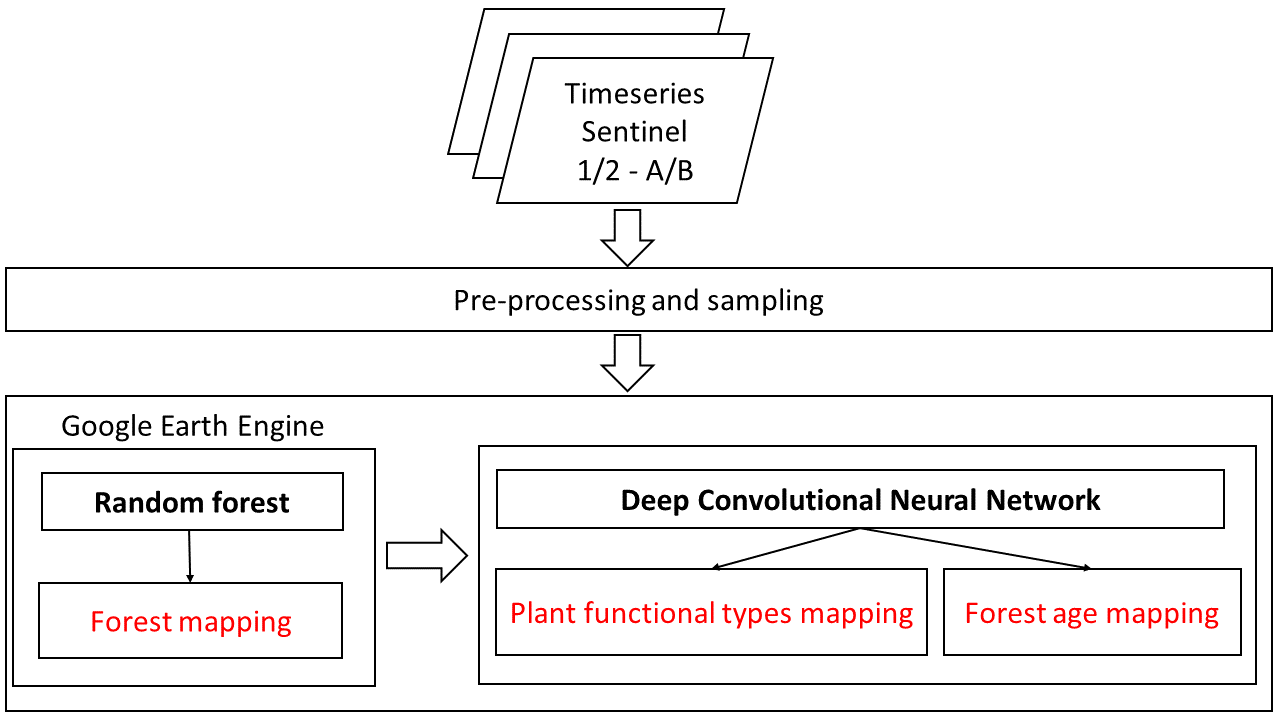
\includegraphics[width=\textwidth]{figs/chap5/workflow.png}
        \caption{Annotations of national forest in Gifu prefecture (black boundary)}
        \label{fig:chap5_studyarea}
    \end{subfigure}

    \begin{subfigure}{\textwidth}
        \centering
        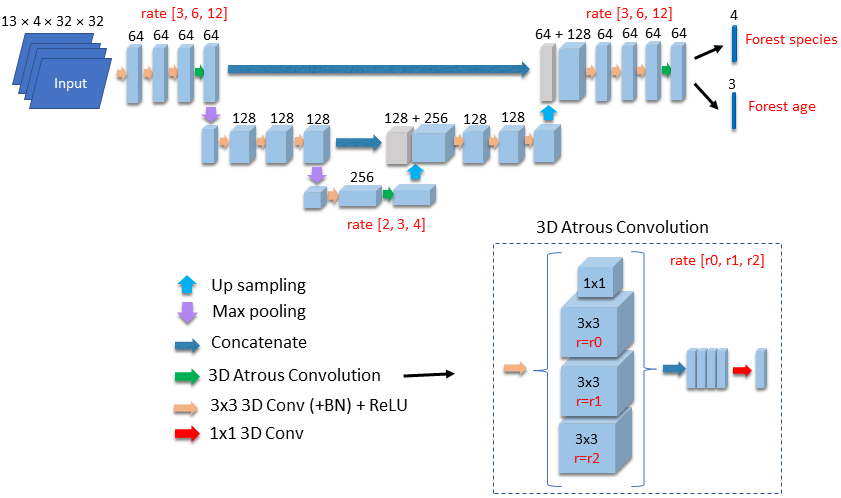
\includegraphics[width=\textwidth]{figs/chap5/model.png}
        \caption{Annotations of national forest in Gifu prefecture (black boundary)}
        \label{fig:chap5_studyarea}
    \end{subfigure}
    \caption[Study area and annotated data]{(a) The designated study area outlined in red is Ena city, (b) demonstrates coarse annotations as an illustrative example, and (c) showcases the corresponding RGB image sourced from Google Earth.}
    \label{fig:chap5_studyarea_gt}
\end{figure}

\subsubsection*{Forest mapping}
In order to quickly map the forest, we deployed the RF model which is a popular ensemble machine learning classifier for land-cover/land-use classification \citep{gislason2006random}. In addition, RF has been proven to be effective in land-cover mapping from low-resolution ground-truth data \citep{robinson2021global}.\par
\subsubsection*{Tree species\slash age mapping}
Although RF is able to perform well with low-resolution labeled data, it is not sufficient to achieve a better result than our proposed deep learning model (Table. 2). The proposed network was designed based on the UNET architecture \citep{ronneberger2015u} and is shallower than the original version (see Fig. 2). We applied 3D Atrous Convolution (3DAConv) to the model as atrous convolution is proven to be effective in semantic segmentation from coarse annotations \citep{chen2017rethinking}. Atrous convolution was introduced in DeepLab architecture \citep{chen2017deeplab} as a term for convolution with upsampled filters. The model backbone is built from encoder and decoder paths. The encoder path consists of three layers. The first one has three 3D convolutions (3DConv) followed by a 3DAConv. The second layer only contains three 3DConvs. The last layer consists of one 3DConv followed by a 3DAConv. A 2$\times$2$\times$2 max pooling layer with strides of two follows each encoder layer. Each 3DConv is followed by a rectified linear unit (ReLU), before each ReLU is a batch normalization (BN). We avoid doubling the number of channels right before the max pooling as introduced in 3D UNET \citep{cciccek20163d}. In the decoder path, the up-convolution (ConvTranspose3D) was applied to upsample the feature map. A 3DAConv was added at the end of decoder path. The output dimensions will be reduced to the number of labels by a 1$\times$1$\times$1 3DConv from the last 3DAConv. The number of labels in our case is 4 for tree species: Broadleaf, Conifer, Cryptomeria, Chamaecyparis obtusa; 3 for tree age: young age ($\le$ 20 years), mature age (21-50 years), harvesting age ($\ge$ 50 years). \par

\begin{table}[tbh!]
    \centering
    \caption[Samples, weights for cross-entropy loss training]{Training and validation samples and the corresponding weights for cross-entropy loss function.}
    \begin{tabular}{c c c c}
    \hline
        Class   & Training set  & Validation set & Weight \\ \hline
        \multicolumn{4}{l}{Tree species (number of input images)} \\ \hline
        Broadleaf   & 5017  & 264  & 0.153 \\ 
        Conifer  & 3048  & 160  & 0.252  \\ 
        Chamaecyparis obtusa   & 3191  & 168  & 0.241 \\ 
        Cryptomeria  & 768  & 40  & 1 \\ \hline
        \multicolumn{4}{l}{Tree age (number of input images)} \\ \hline
        Harvesting age   & 4000  & 205  & 0.05 \\ 
        Mature age  & 2095  & 110  & 0.1  \\ 
        Young age   & 186  & 10 & 1 \\ \hline
    \end{tabular}
    \label{tab:chap5_tab1}
\end{table}

\subsubsection*{Experiment design and settings}
For tree species/age mapping, we designed the following experiment to evaluate the performance of the proposed network with the RF, 2D, 3D UNET, and our model. The time-series satellite data of Sentinel 1, 2 in 2018 was organized into three periods: January-April (P1), May-August (P2), October-December (P3). For each period, the satellite image was mosaicked and composited. We first investigate the effect of seasonal changes on the performance of tree species/age mapping from satellite data employing RF and 2D UNET. Due to the input shape constraint, we only can examine the performance of 3D UNET and the proposed model with the data of the entire year.  In order to train the data with our network or 3D UNET, the input shape must be 13$\times$4$\times$32$\times$32. In doing so, the DEM band was stacked to the Sentinel 1/2 in P1, P2, P3 (each 13$\times$32$\times$32) to make the input trainable to the network. \par
To evaluate the performance of the segmentation models, we used overall accuracy (OA) score on the validation set. Finally, the results map obtained by each model were generated for visual examination. \par
We implemented the deep learning model in Pytorch and trained the model on NDVIA GeForce RTX 3080 Ti GPU. The model was trained with 100 epochs and was optimized by Adam optimizer with the initial learning rate 10\textsuperscript{-5}. The learning rate is divided by 2 after every 10 epochs.\par
For forest mapping, the implementation is directly supported in the GEE API which effortlessly enhances the computing performance for mapping stages. \par

\section{Experimental results} \label{chap5_result}
For forest mapping, only Sentinel 2 in June 2018 with 10m-resampled DEM data derived from GEE were used to train the RF classifier as by our observation, June data has least slope effect in regions with high elevations. The model achieved 94.5\% OA for forest/non-forest classification. The forest map produced by the model is shown in Fig. 3. \par

\begin{table}[tbh!]
    \centering
    \caption{The experimental results of UNET and our model.}
    \begin{tabular}{cccc}
    \hline
        \multirow{2}{*}{Model} & \multirow{2}{*}{Time-series period} & \multicolumn{2}{c}{Highest OA (\%)} \\ \cline{3-4}
        ~ & ~ & Species & Age \\ \hline
        \multirow{3}{*}{RF} & P2 & 67.41 & 73.94 \\ 
        ~ & P1 + P2 & 71.68 & 78.66 \\ 
        ~ & P1 + P2 + P3 & 71.65 & 78.68 \\ \hline
        \multirow{3}{*}{2D UNET} & P2 & 59.81 & 65.67 \\ 
        ~ & P1 + P2 & 67.25 & 75.4 \\ 
        ~ & P1 + P2 + P3 & 65.02 & 74.55 \\ \hline
        3D UNET & P1 + P2 + P3 & 76.91 & 80.53 \\ 
        Our model & P1 + P2 + P3 & 77.80 & 81.74 \\ \hline
    \end{tabular}
    \label{tab:chap5_tab2}
\end{table}


\begin{figure}[tbh!]
    \centering
    \includegraphics[width=\textwidth]{figs/chap5/Forest.png}
    \caption{Forest map in Ena City, Japan.}
    \label{fig:chap5_fig3}
    
\end{figure}

\begin{figure}[p]
    \centering
    \begin{subfigure}{\textwidth}
        \centering
        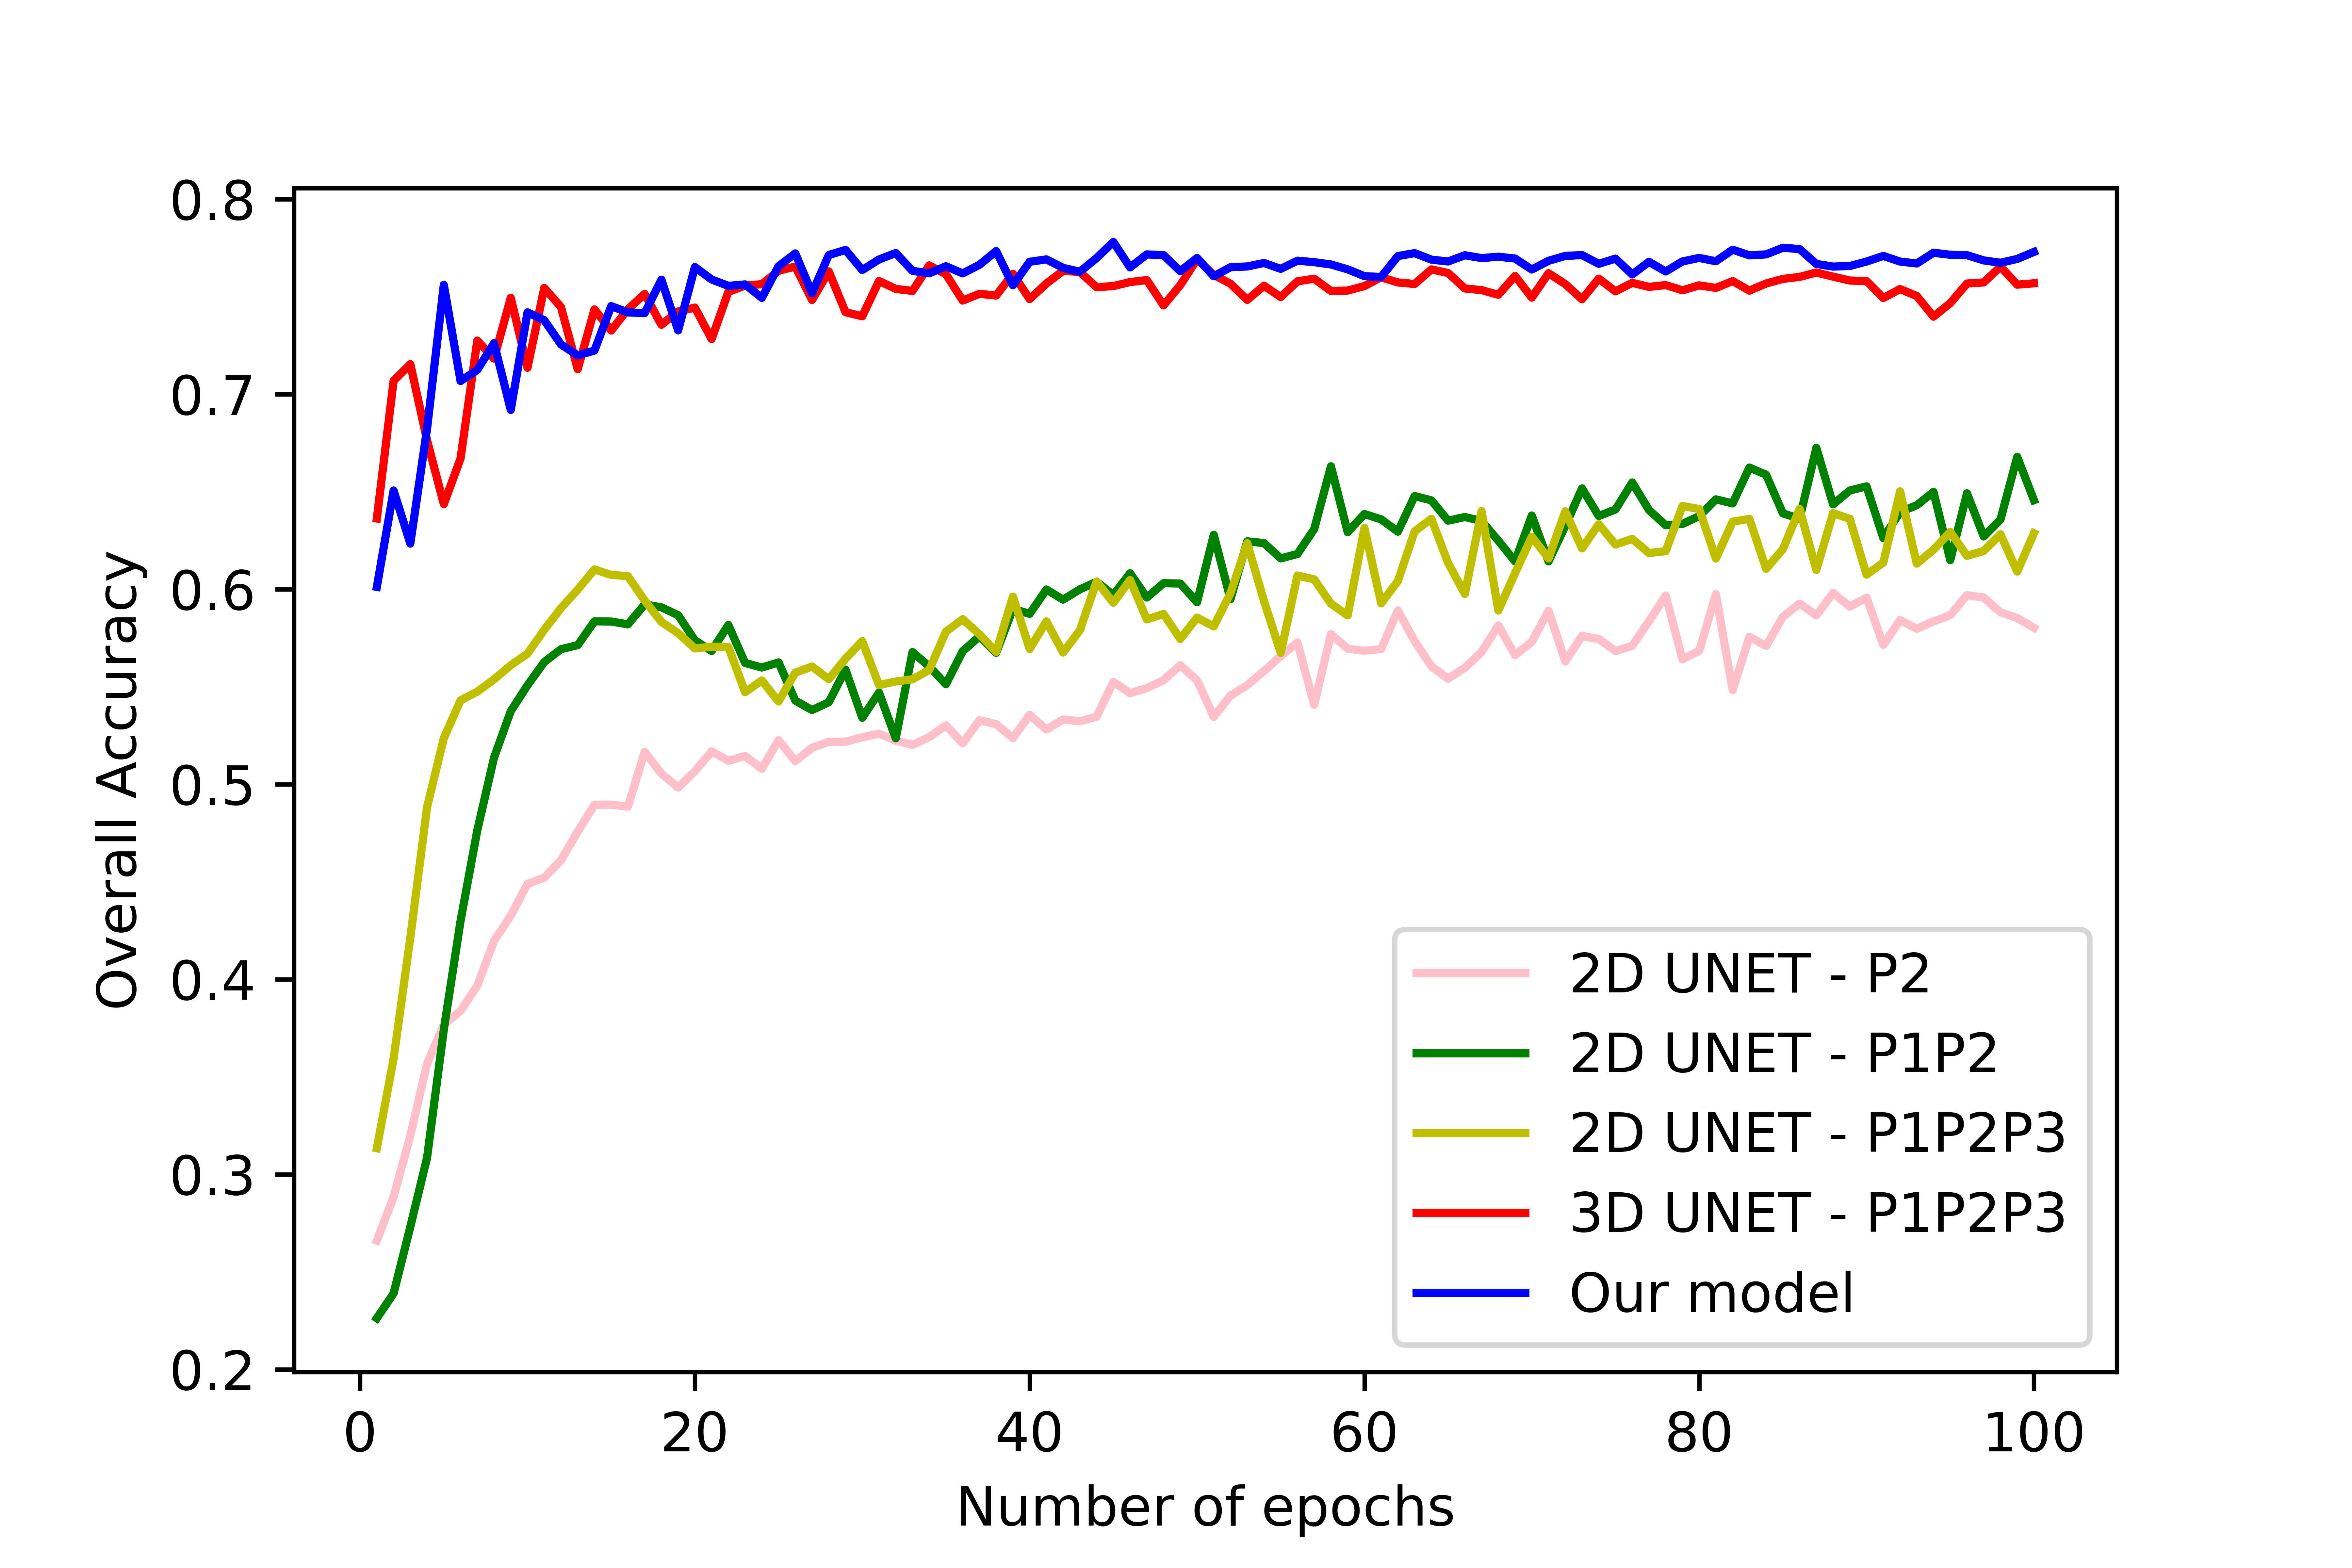
\includegraphics[width=\textwidth]{figs/chap5/spec_acc.png}
        \caption{Tree species segmentation.}
        \label{fig:chap5_fig4}
    \end{subfigure}

    \begin{subfigure}{\textwidth}
        \centering
        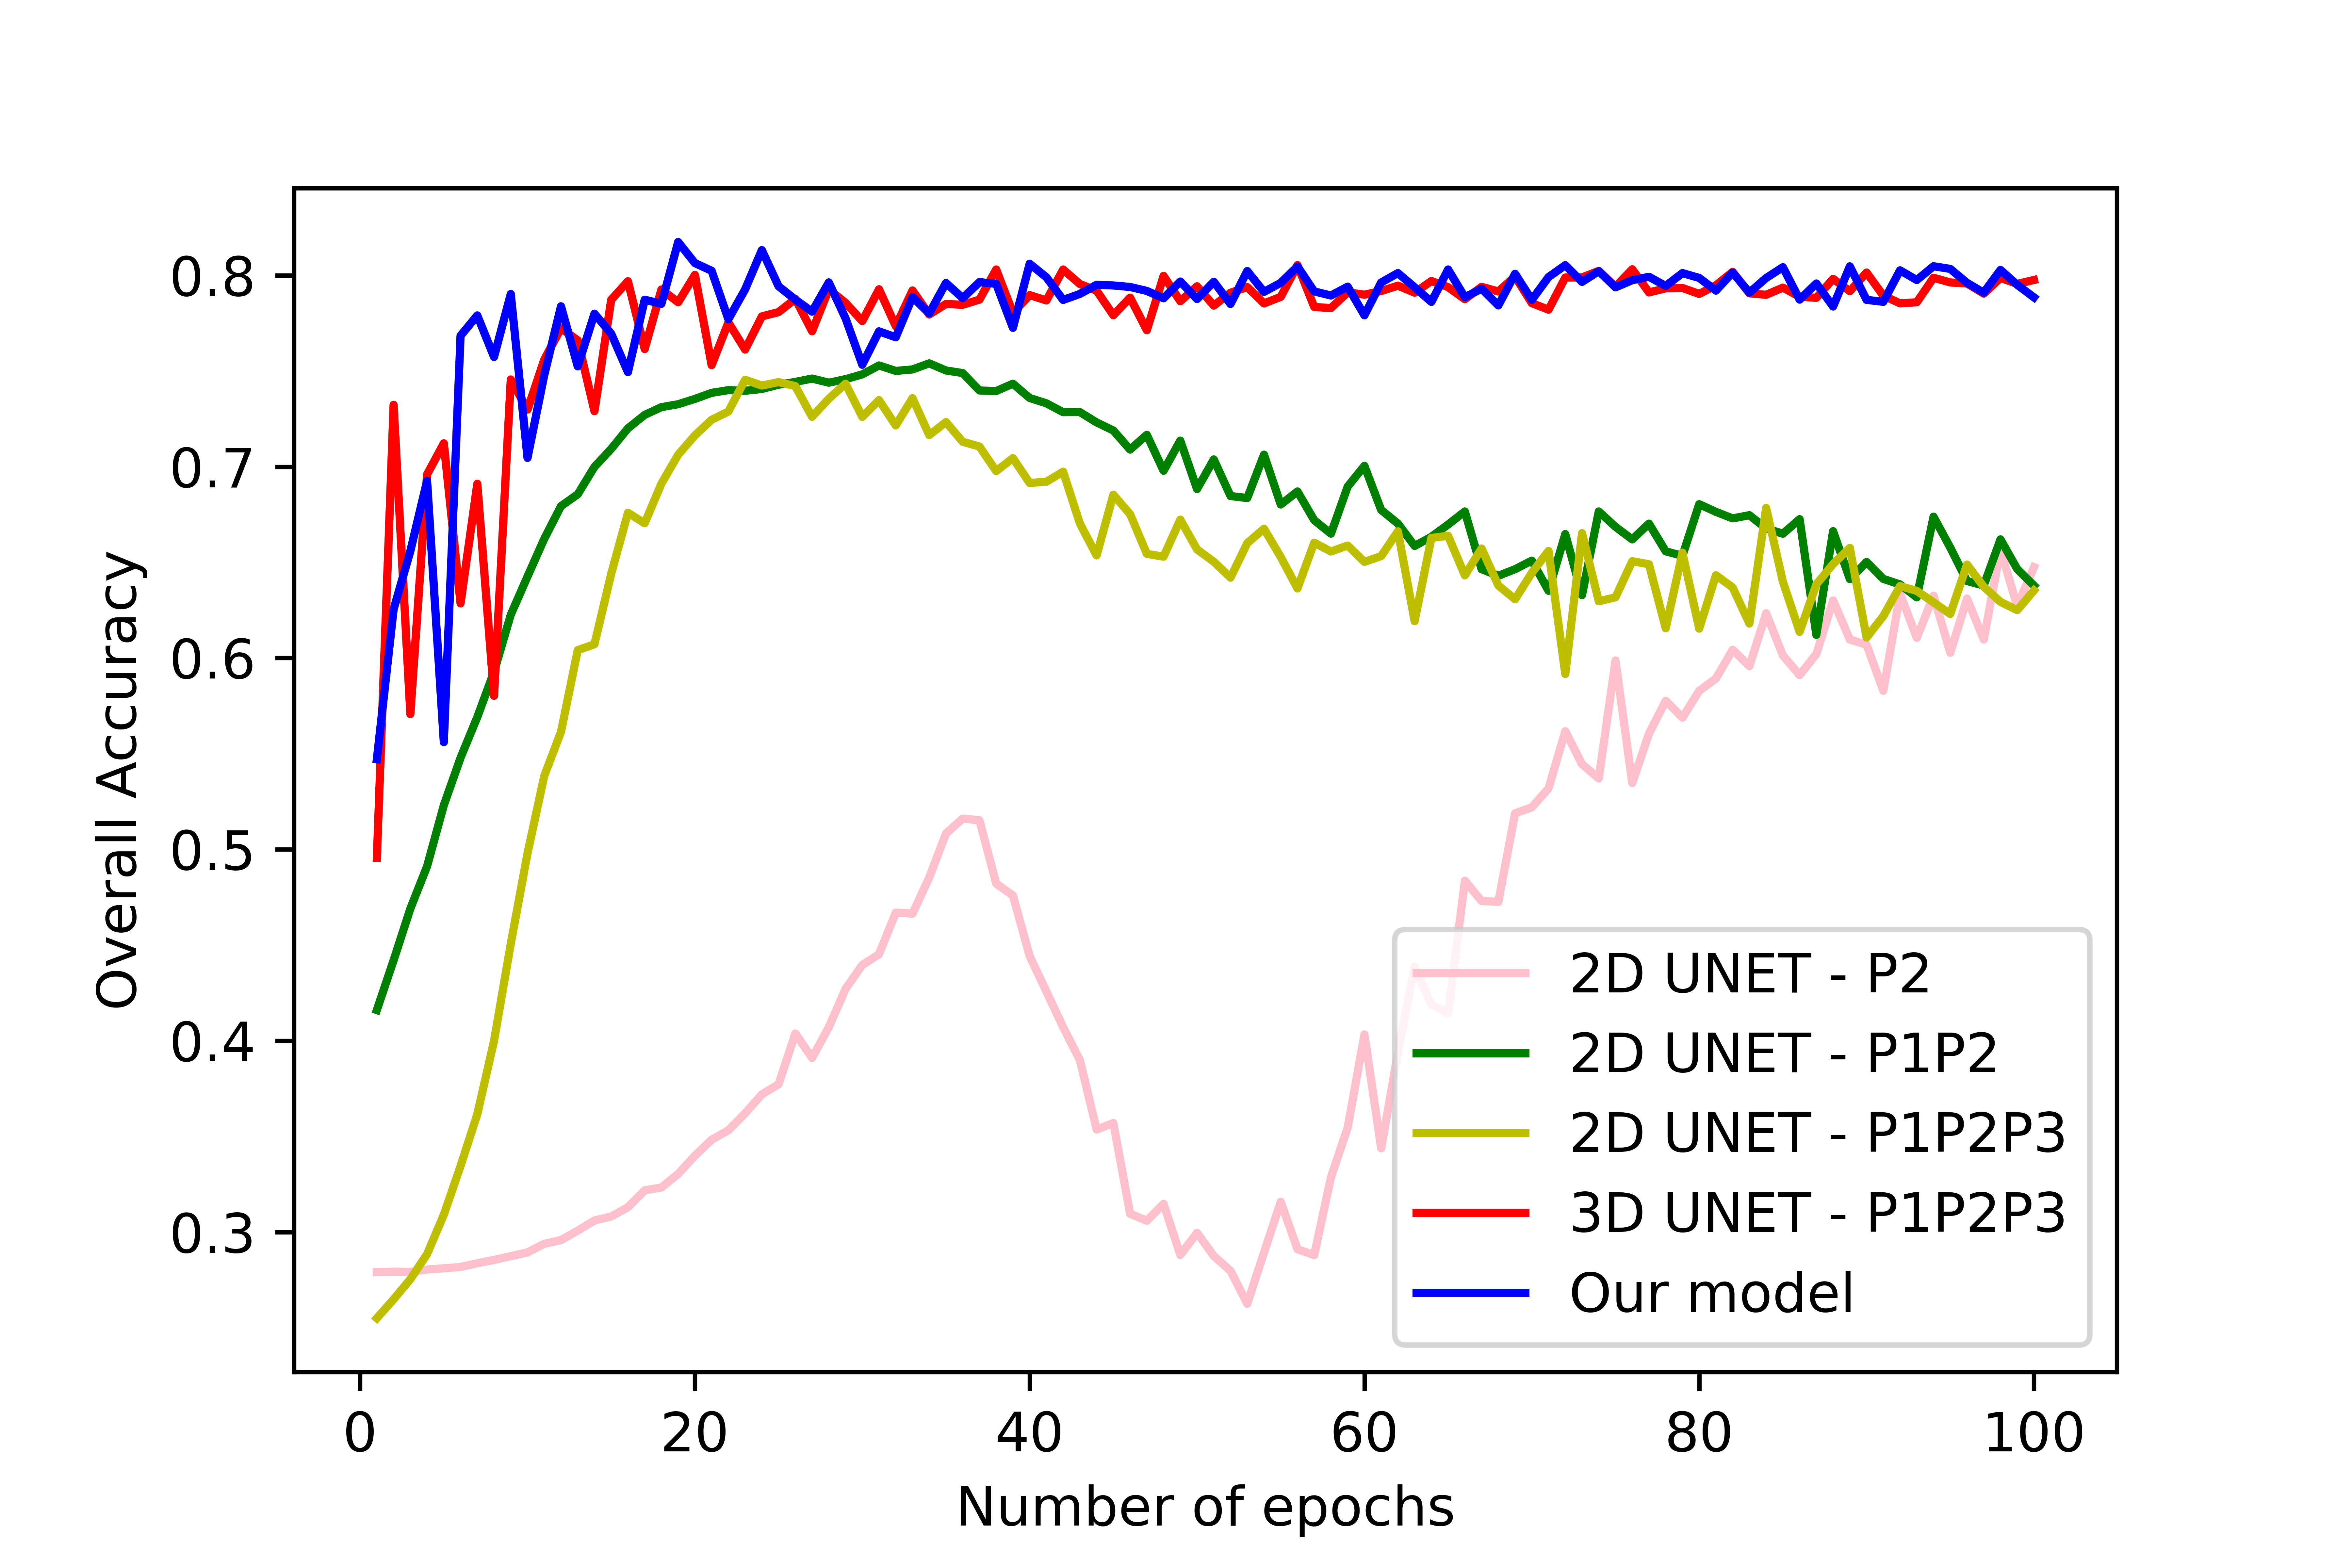
\includegraphics[width=\textwidth]{figs/chap5/age_acc.png}
        \caption{Tree age segmentation.}
        \label{fig:chap5_fig5}
    \end{subfigure}
    \caption[Study area and annotated data]{OA profile of tre species (a) and tree age (b) segmentation}
    \label{fig:chap5_fig45}
\end{figure}

As observed from Table. 2, RF outperformed 2D UNET in all the tests. Both RF and 2D UNET experiments had a certain outcome that employed only P2 period resulting in the lowest OA in both species and age segmentation. The OA is significantly improved when a longer time-series scheme is adopted from P2 to P1 + P2. Adding P3 to the training set did not enhance the performance of RF and 2D UNET compared to P1 + P2. That means, in terms of utilizing time-series data for forest species/age segmentation in the study area, it would be preferable to use the data collected from January to August period with an ensemble learning model from multiple decision trees like RF or a 2D UNET-based CNN architecture.\par

Despite a minor effect of P3 data to the performance of RF and 2D UNET, with 3D CNN scheme in 3D UNET and our suggested model, incorporating P3 data has essentially increased the OA of tree species/age discrimination. The performance of our model and 2D/3D UNET in 100 epochs is presented in Table. 2, Fig. 4, and Fig. 5. The OA has importantly improved from 71.68\% to 76.91\% with 3D UNET, 77.80\% with our model for tree species segmentation, and from 78.66\% to 80.53\% with 3D UNET, 81.74\% with our model for tree age segmentation. \par
The OA profiles in Table. 2, Fig. 4, and Fig. 5 show that our model out-performed RF, 2D UNET and 3D UNET by approximately 6.12\%, 10.55\%, 0.89\% OA for tree species and 3.03\%, 6.31, 1.18\% OA for tree age segmentation, respectively. \par
Fig. 6 is the tree age map produced by our model. The major harvesting-age area was inferred to be mostly located in the Northern, Southern, and central parts of the city. The major mature-age forest is distributed throughout the region while small areas of young-age forest are observed scattering over the city from the west to the south. \par
\begin{figure}[tbh!]
    \centering
    \includegraphics[width=\textwidth]{figs/chap5/age_map.png}
    \caption[Inferred tree age map in Ena City]{Inferred tree age map in Ena City, Japan – 2018.}
    \label{fig:chap5_fig6}
\end{figure}
The inferred tree species map is illustrated in Fig. 7. Chamaecyparis obtusa is the most dominant tree and is distributed all over the region. Cryptomeria is predominantly occupied in the central Southeast and Northwest part of the study area. The majority of Broadleaf are mostly allocated in the Northeast, Southern, and Northwest parts of the region. The detected Conifer is scattered in the area in the Northern and Southern parts, a minor contribution comes from the Northwest of the city \par
\begin{figure}[tbh!]
    \centering
    \includegraphics[width=\textwidth]{figs/chap5/spec_map.png}
    \caption[Inferred tree species map in Ena City]{Inferred tree species map in Ena City, Japan – 2018.}
    \label{fig:chap5_fig7}
\end{figure}

\section{Conclusion} \label{chap5_conclusion}
In this study, by utilizing remote sensing, RF classifier, and deep learning, the approach for forest-related SDG issues monitoring in data-scarce regions has been proposed. We examined the approach in Ena City, Japan and achieved promising results in forest mapping, and tree species/age mapping. Our proposed model outperforms the RF, 2D/3D UNET in tree species/age segmentation with coarse-polygonal ground-truth data. The outcome of this study could be served as an input for further steps to produce high-resolution land cover map for the data-scarce regions. In the future, we will investigate the postprocessing method to improve the map quality from coarse annotations.